\documentclass[10pt]{beamer}
\setbeamersize{description width=2em}
\setbeamertemplate{navigation symbols}{\vspace{-2ex}}
\usefonttheme{serif}
\usepackage{mathpazo}
\usepackage{pifont}
\usepackage{pgfplots}
\usepackage{ragged2e}
\usepackage{tikz}
\usepackage{bm}
\usepackage{marvosym}
\usepackage{xcolor}
\usepackage{caption,subcaption}
\usepackage[most]{tcolorbox} % added for ovalbox
\newcounter{savefootnote}% Save footnote counter
\usepackage{xmpmulti}

\usepackage{media9}



\usepackage{dblfnote}
\DFNalwaysdouble % for this example


\usetikzlibrary{arrows.meta}


\usepackage[edges]{forest}

\usepackage[sfdefault,condensed]{roboto}


\title[HPC/AI Days]{\textcolor{um6pcolor}{HPC: Accelerating Progress in CFD}}

\author[Radouan Boukharfane]{\underline{Radouan Boukharfane}}
\institute[UM6P]{Mohammed VI Polytechnic University (UM6P), Benguerir, Morocco \\ \begin{center}
\includegraphics[height=2cm]{figs/logo-um6p-black.png}
\includegraphics[height=2.5cm]{figs/logo_um6p.png}
\end{center}}
\date{\underline{UM6P, Benguerir, 29th April 2024} \\ \bigskip \textcolor{um6pcolor}{HPC/AI Days}}

\usepackage{caption}
\captionsetup[figure]{labelformat=empty}
\setbeamercolor{frametitle}{fg=white,bg=um6pcolor} %section slide title
\setbeamercolor{section in foot}{fg=white, bg=um6pcolor} % footsections
\setbeamercolor{part title}{fg=white, bg=um6pcolor}
\setbeamertemplate{footline}
{
\hbox{%
\begin{beamercolorbox}[wd=.33\paperwidth,ht=2.6ex,dp=1ex,left,leftskip=2ex]{section in foot} % footsection 1
\usebeamerfont{section in foot} \insertshortauthor
\end{beamercolorbox}%
\begin{beamercolorbox}[wd=.33\paperwidth,ht=2.6ex,dp=1ex,center]{section in foot} % footsection 2
\usebeamerfont{section in foot} Page: \insertframenumber/\inserttotalframenumber
\end{beamercolorbox}%
\begin{beamercolorbox}[wd=.34\paperwidth,ht=2.6ex,dp=1ex,right,rightskip=2ex]{section in foot}
\usebeamerfont{section in foot} HPC/AI Days Workshop 
\end{beamercolorbox}}%
\vskip0pt%
}


\setbeamertemplate{section page}{
\centering
\begin{columns}
\begin{column}{\paperwidth}
\begin{beamercolorbox}[sep=12pt,center]{part title}
\usebeamerfont{section title}\insertsection\par
\end{beamercolorbox}
\end{column}
\end{columns}
}

\usepackage{xcolor}

\definecolor{um6pcolor}{RGB}{216,73,43}


\setbeamercolor{structure}{fg=um6pcolor}

\usecolortheme[light]{solarized}



\newcommand{\pd}[3][]{\frac{\partial^{#1}#2}{\partial{#3}^{#1}}}
\newcommand{\lrbkt}[1]{\left( #1 \right)}                         % (.)


\begin{document}


\begin{frame}[plain]
\titlepage
\end{frame}

\begin{frame}{Overview}
\tableofcontents
\end{frame}

\section{Introduction to HPC for CFD}

\begin{frame}{Outline}
\tableofcontents[currentsection]
\end{frame}

\subsection{What is CFD?}

\begin{frame}{What is CFD?}
\begin{itemize}
\justifying
\item[\ding{113}] Fluid dynamics
\begin{itemize}
\justifying
\item[\ding{252}] Fluid dynamics is a subdiscipline of fluid mechanics that describes the flow of fluids.
\item[\ding{252}] Fluid flow is commonly studied in one of three methods:
\begin{itemize}
\justifying
\item[\ding{250}] Analytical methods
\item[\ding{250}] Experimental methods
\item[\ding{250}] Numerical methods: Computational fluid dynamics (CFD)
\end{itemize}
\end{itemize}
\end{itemize}

\begin{itemize}
\justifying
\item[\ding{113}] What is CFD?
\begin{itemize}
\justifying
\item[\ding{252}] Computational fluid dynamics (CFD) is a branch of fluid mechanics that uses numerical analysis and data structures to analyze and solve problems that involve fluid flows.
\item[\ding{252}] Key governing equations: Navier-Stokes equation, Continuity equation, energy equation.
\item[\ding{252}] Numerical methods: Finite Difference Method (FDM), Finite Element Method FEM), Finite Volume Method (FVM), ...
\end{itemize}
\end{itemize}
\end{frame}

\begin{frame}{What is CFD?}


\def\firstcircle{(0,0) circle (2.6cm)}
\def\secondcircle{(60:3cm) circle (2.6cm)}
\def\thirdcircle{(0:3cm) circle (2.6cm)}
\begin{figure}
\centering
\begin{tikzpicture}
\begin{scope}[shift={(6cm,-10cm)}, fill opacity=0.3]
% Drawing black outlines for the circles
\draw[black, line width=1.0pt] \firstcircle;
\draw[black, line width=1.0pt] \secondcircle;
\draw[black, line width=1.0pt] \thirdcircle;
% Filling the circles with color
\fill[solarizedCyan]    \firstcircle;
\fill[solarizedYellow]  \secondcircle;
\fill[solarizedMagenta] \thirdcircle;
\node[align=center, text opacity=1] at (-1.2, 0.4) {\underline{\bf\textsc{\scriptsize Applied Mathematics}}};
\node[align=center, text opacity=1] at (-0.65, -0.5) {\tiny Mathematical modeling};
\node[align=center, text opacity=1] at (-0.65, -0.7) {\tiny Convergence Acceleration};
\node[align=center, text opacity=1] at (-0.65, -0.9) {\tiny Stability \& Convergence Analysis};
\node[align=center, text opacity=1] at (-0.65, -1.1) {\tiny Uncertainty Quantification};
\node[align=center, text opacity=1] at (1.4,4) {\underline{\bf\textsc{\scriptsize Computer Science}}};
\node[align=center, text opacity=1] at (1.5,3.5) {\tiny\ Solver/Software development};
\node[align=center, text opacity=1] at (1.5,3.3) {\tiny High-performance computing};
\node[align=center, text opacity=1] at (1.5,3.1) {\tiny Parallel \& Distributed Computing};
\node[align=center, text opacity=1] at (1.5,2.9) {\tiny Code Verification \& Validation};
\node[align=center, text opacity=1] at (4.15,0.4) {\underline{\bf\textsc{\scriptsize Engineering Science}}};
\node[align=center, text opacity=1] at (3.7,-0.5) {\tiny Turbulence Modeling};
\node[align=center, text opacity=1] at (3.7,-0.7) {\tiny Heat Transfer Analysis};
\node[align=center, text opacity=1] at (3.7,-0.9) {\tiny Fluid-Structure Interaction};
\node[align=center, text opacity=1] at (3.7,-1.1) {\tiny Design Optimization};
\node[align=center, text opacity=1] at (1.5,-0.8) {\tiny\rotatebox{90}{Problem formulation}};
\node[align=center, text opacity=1] at (3.0,1.55) {\tiny\rotatebox{30}{Data Visualization}};
\node[align=center, text opacity=1] at (0.0,1.7) {\tiny\rotatebox{-30}{Numerical Methods}};
\node[align=center, text opacity=1] at (1.45,0.95) {\bf\textsc{CFD}};
\end{scope}
\end{tikzpicture}
\end{figure}
\end{frame}

\subsection{Why use CFD?}


\begin{frame}{Why use CFD?}

\begin{itemize}
\justifying
\item[\ding{113}] Numerical solutions
\begin{itemize}
\justifying
\item[\ding{252}] Analytical solutions of some Patial Differential Equations (PDEs) cannot be obtained currently. So Analytical methods are limited to simplified cases
such as solving 1D or 2D geometry, 1D flow, and steady flow.
\end{itemize}
\item[\ding{113}] Relatively low cost
\begin{itemize}
\justifying
\item[\ding{252}] Experimental methods need a lot of resources such as electricity, expensive equipment, data monitoring, and data post-processing.
\justifying
\item[\ding{252}] CFD simulations are relatively inexpensive, and costs are likely to decrease as computers become more powerful.
\end{itemize}
\item[\ding{113}] Ability to simulate any conditions
\begin{itemize}
\justifying
\item[\ding{252}] CFD provides the ability to theoretically simulate any physical condition.
\end{itemize}
\item[\ding{113}] Comprehensive information
\begin{itemize}
\justifying
\item[\ding{252}] CFD allows the analyst to examine a large number of locations in the region of interest, and yields a comprehensive set of flow parameters for examination.
\end{itemize}
\end{itemize}
\end{frame}

\subsection{Where is CFD used?}

\begin{frame}{Where is CFD used?}

\begin{columns}
\begin{column}{0.4\textwidth}
\begin{itemize}
\item[\ding{113}] \textbf{CFD is used in}:
\begin{itemize}
\justifying
\item[\ding{252}] Aerospace
\item[\ding{252C}] Automotive
\item[\ding{252}] Chemical Processing
\item[\ding{252}] Hydraulics
\item[\ding{252}] Marine
\item[\ding{252}] Oil \& Gas
\item[\ding{252}] Power Generation
\item[\ding{252}] Weather forecasting
\item[\ding{252}] Ocean
\item[\ding{252}] ...
\end{itemize}
\end{itemize}
\end{column}
\begin{column}{0.7\textwidth}
\includegraphics[height=0.15\columnwidth,width=2.0cm]{./figs/app1.jpg}
\includegraphics[height=0.15\columnwidth,width=2.0cm]{./figs/app2.jpg}
\includegraphics[height=0.15\columnwidth,width=2.0cm]{./figs/app3.jpg}\\
\includegraphics[height=0.15\columnwidth,width=2.0cm]{./figs/app4.jpg}
\includegraphics[height=0.15\columnwidth,width=2.0cm]{./figs/app5.jpeg}
\includegraphics[height=0.15\columnwidth,width=2.0cm]{./figs/app6.jpg}\\
\includegraphics[height=0.20\columnwidth,width=3.05cm]{./figs/app13.png}
\includegraphics[height=0.20\columnwidth,width=3.05cm]{./figs/app14.jpg}\\
\includegraphics[height=0.15\columnwidth,width=2.0cm]{./figs/app7.jpeg}
\includegraphics[height=0.15\columnwidth,width=2.0cm]{./figs/app8.jpeg}
\includegraphics[height=0.15\columnwidth,width=2.0cm]{./figs/app9.jpeg}\\
\includegraphics[height=0.15\columnwidth,width=2.0cm]{./figs/app10.jpg}
\includegraphics[height=0.15\columnwidth,width=2.0cm]{./figs/app11.jpg}
\includegraphics[height=0.15\columnwidth,width=2.0cm]{./figs/app12.jpg}\\
\end{column}
\end{columns}

\end{frame}


\subsection{Why use HPC for CFD?}

\begin{frame}{Why use HPC for CFD?}
\begin{itemize}
\justifying
\item[\ding{113}] CFD: A Leading consumer of High-Performance Computing

\item[\ding{113}] Speed
\begin{itemize}
\justifying
\item[\ding{252}] With the help of HPC, CFD simulations can be executed in a short period of time, which means engineering data can be introduced early in the design process.
\end{itemize}
\it
\item[\ding{113}] Memory
\begin{itemize}
\justifying
\item[\ding{252}] A large CFD simulation can’t typically fit into the memory of a single machine.
\end{itemize}
\end{itemize}
\end{frame}


\subsection{Where is CFD headed in light of NASA2030's vision?}

\begin{frame}{Where is CFD headed in light of NASA2030's vision?}
\begin{figure}
\centering
\includegraphics[width=0.99\textwidth]{figs/nasa.png}
\begin{tikzpicture}[remember picture,overlay]
% \draw [black, line width=2pt] (current page.north west) ++(8.6cm,-6.2cm) rectangle ++(1.55cm,-0.5cm);
% \draw [black, line width=2pt] (current page.north west) ++(3.4cm,-4.8cm) rectangle ++(2.1cm,-0.5cm);
\end{tikzpicture}
\end{figure}
\end{frame}


\subsection{What are the main CFD methods?}

\begin{frame}{What are the main CFD methods?}

\begin{equation}
\resizebox{0.91\hsize}{!}{
$
\left\{
\begin{aligned}
\pd{\overline{\rho}}{t}+\pd{\overline{\rho} \widetilde{u}_i}{x_i}&=0
\\
\pd{\overline{\rho} \widetilde{u}_i}{t}+
\pd{\overline{\rho}\widetilde{u}_i\widetilde{u}_j}{x_j}&=-\pd{\overline{p}}{x_i}+\pd{\check{\tau}_{ij}}{x_j}
-\pd{\tau_{ij}^{\mathrm{sgs}}}{x_j}
+\pd{}{x_j}\lrbkt{\overline\tau_{ij}-\check\tau_{ij}}
\\
\pd{\overline{\rho} \widetilde{Y}_\alpha}{t} 
+\pd{\overline{\rho} \widetilde{Y}_\alpha \widetilde{u}_i}{x_i}
&   = -\pd{\check J_{\alpha i}}{x_i}
- \pd{J_{\alpha i}^{\mathrm{sgs}}}{x_i} 
- \pd{}{x_i} \lrbkt{\overline J_{\alpha i}-\check J_{\alpha i}}
+ \overline{\rho}\widetilde{\dot\omega}_\alpha
\\
\pd{\bar\rho \check e_t}{t} 
+\pd{\bar{\rho} \check e_t \tilde{u}_j}{x_j}
& = - \pd{\bar{p}\tilde{u}_j}{x_j}
+ \pd{\check\tau_{ij}\tilde u_i}{x_j}
- \pd{\check{q}_j}{x_j}
- (B_1 + B_2 + B_3)
+ (B_4 + B_5 + B_6)
- B_7
\end{aligned}
\right.
$}
\end{equation}

with 
%

\begin{equation}
\resizebox{0.31\hsize}{!}{
$
\left\{
\begin{aligned}
   B_1 &= \pd{}{x_j}(\bar{eu_j}-\tilde e\tilde u_j) 
%        \approx \frac{1}{\gamma-1}\pd{}{x_j}(\bar{pu_j}-\bar p\tilde u_j)
        \approx \pd{\tilde c_v\theta_j^{\mathrm{sgs}}}{x_j}
\\
   B_2 &= \bar{p\pd{u_j}{x_j}}-\bar p\pd{\tilde u_j}{x_j}=\Pi_{\mathrm{dil}}^{\mathrm{sgs}}\\
   B_3 &= \pd{}{x_j}(\tau_{ij}^{\mathrm{sgs}}\tilde u_i) \\
   B_4 &= \tau_{ij}^{\mathrm{sgs}}\pd{}{x_j}\tilde u_i \\
   B_5 &= \bar{\tau_{ij}\pd{}{x_j}u_i}-\bar\tau_{ij}\pd{}{x_j}\tilde u_i=\epsilon_v^{\mathrm{sgs}}
\end{aligned}
\right.
$}
\end{equation}

%


\end{frame}


\begin{frame}{What are the main CFD methods?}


\begin{figure}
\centering
\includegraphics[width=0.99\textwidth]{/home/rb/Desktop/pics1-modified.png}
\begin{tikzpicture}[remember picture,overlay]
\node[align=center, text opacity=1] at (-2.2,4.7) {$\mathcal{R}e^{9/4}$ grids};
\node[align=center, text opacity=1] at (-1.3,3.) {$\mathcal{R}e^{9/5}$ grids};
\node[align=center, text opacity=1] at (-0.2,1.5) {$log(\mathcal{R}e)$ grids};
\end{tikzpicture}
\end{figure}

$^{\ast}\mathcal{R}e$ is a measure of turbulence intensity. 


\end{frame}



\begin{frame}{What are the main CFD methods?}

\begin{figure}
\centering
\includegraphics[width=0.6\textwidth,angle=-90]{/home/rb/Desktop/flame-modified.png}
\begin{tikzpicture}[remember picture,overlay]
\node[align=center, text opacity=1] at (-6,-5.2) {\Large DNS};
\node[align=center, text opacity=1] at (-6,-2.9) {\Large LES};
\node[align=center, text opacity=1] at (-6,-1.1) {\Large RANS};

\node[align=left, text opacity=1] at (0.8,-5.2) {\Large $\mathcal{O}\left(\mathcal{R}e^{3}\right)$};
\node[align=right, text opacity=1] at (1.6,-2.9) {\Large $\mathcal{O}\left(\mathcal{R}e^{2}-\mathcal{R}e^{2.5}\right)$};
\node[align=center, text opacity=1] at (0.8,-1.1) {\Large $\mathcal{O}\left(\mathcal{R}e\right)$};

\end{tikzpicture}
\end{figure}

Need for more computing power in turbulence simulations relevant to high $\mathcal{R}e$ continues... 
\end{frame}


\section{LES of Wakes of Wind Turbines Operating in Turbulent Inflow}

\begin{frame}{Outline}
\tableofcontents[currentsection]
\end{frame}



\begin{frame}{Context}

\begin{itemize}
\justifying
\item[\ding{113}] The global energy challenge:
\begin{itemize}
\justifying
\item[\ding{252}] Energy supply stability
\item[\ding{252}] Climate change
\end{itemize}

\item[\ding{113}] \textbf{Increasing demand} for renewable energies: there is a need to increase electrical output and reduce the LCOE\footnote[frame]{\tiny\color{um6pcolor} Veers, P. et al. (2017). Science}.

\item[\ding{113}] Morocco has \textbf{favorable climatic and geographic conditions} for installing wind turbines.
\begin{itemize}
\justifying
\item[\ding{252}] Wind generation potential of 5000 TWh per year
\item[\ding{252}] Useful capacity of 25,000 MW
\end{itemize}
\end{itemize}

\noindent\makebox[\linewidth]{\rule{\paperwidth}{0.4pt}}

\begin{columns}
\begin{column}{0.6\textwidth}
\begin{itemize}
\item[\ding{113}] \textbf{New challenges}:
\begin{itemize}
\justifying
\item[\ding{252}] Larger rotors with flexible blades
\item[\ding{252}] Complexity of servo-hydro-aero-elasticity
\item[\ding{252}] Use of high-fidelity simulations to capture complexe phenomena (i.e. dynamic wake meandering, wake steering, blade loading cycles to include wake turbulence,...).
\end{itemize}
\end{itemize}
\end{column}
\begin{column}{0.4\textwidth}
\begin{tikzpicture}
\node[anchor=south west,inner sep=0] (image) at (0,0) {\includegraphics[width=0.99\columnwidth]{./figs/windMorocco.jpeg}};
\draw[-,very thick, um6pcolor] (image.north west) -- (image.north east) node[midway,above] {\tiny Offshore turbines. Photo: Xlinks};
\end{tikzpicture}
\end{column}
\end{columns}
\end{frame}


\begin{frame}{Context}
\begin{block}{}
\begin{itemize}
\justifying

\bigskip
\item[\ding{113}] Large-Eddy Simulation is a promising tool for predicting wind turbine performances as it provides access to unsteady flow features.
\item[\ding{113}] Simulating the aerodynamics of an operating wind turbine at a high fidelity level is a challenging task due to the extremely high Reynolds number involved.
\begin{itemize}
\justifying
\item Develop a computational in-house parallel solver at UM6P.
\item Implement a hybrid approach combining Large Eddy Simulation (LES) and Actuator Line Modeling (ALM) techniques.
\item Enhance accuracy in predicting the flow field and aerodynamic loading on turbine blades.
\item Achieve advantages over a pure LES approach, such as optimal workload balacing and return time. 
\end{itemize}

\end{itemize}
\end{block}

\end{frame}

\subsection{Presentation of the numerical framework}

\begin{frame}{Overview of the Numerical Solver}
\begin{itemize}
\item[\large\ding{113}] The numerical framework is an in-house finite volume solver designed for incompressible flows and massively parallel computations.
\begin{itemize}
\item[\large\ding{52}] IO formats: Fluent, Ensight, prepartionned HDF5 (XDMF) with compression
\item[\large\ding{52}] Partitioned mesh support for HDF5 independent of the number of processors
\item[\large\ding{52}] Parallel interpolator for partitioned HDF5 meshes
\end{itemize}
\item[\large\ding{113}] Utilizes a Projection Method Based on Fractional Time Steps, developed by Chorin\footnote[frame]{\tiny\color{um6pcolor} Chorin, A. J. (1968). Mathematics of Computation.}, and Improved by Kim \& Moin\footnote[frame]{\tiny\color{um6pcolor} Kim, J., \& Moin, P. (1985). Journal of Computational Physics.}.
\begin{itemize}
\item[\large\ding{52}] Highly efficient Deflated Preconditioned Conjugate Gradient: Use of a residual recycling method and an adaption of convergence criteria.
% \item[\large\ding{52}] Fourth-order central scheme is employed for spatial integration to reduce dissipation and dispersion errors.
\end{itemize}
\item[\large\ding{113}] Turbulence model implemented: Constant Smagorinsky, Localized dynamic Smagorinsky, Vreman, WALE, $\sigma$-model.
\item[\large\ding{113}] It Implements two levels of parallelism to enable massively parallel computations:
\begin{itemize}
\item[\large\ding{52}] Single Domain Decomposition.
\item[\large\ding{52}] Double Domain Decomposition.
\end{itemize}
\end{itemize}
\end{frame}

%\subsection{tion{Mesh Management in {IZEM}}

\begin{frame}{Mesh Management on Processors}
\begin{itemize}
\item[\large\ding{113}] {\color{um6pcolor}First Level}: Single-Level Domain Decomposition
\item[\large\ding{113}] Utilization of {\color{um6pcolor}Metis} and {\color{um6pcolor}Scotch} for Mesh Partitioning: Ensuring optimal workload distribution is essential.
\item[\large\ding{113}] Implementation of {\color{um6pcolor}MPI library} for Processor Information Exchange at Interfaces
\begin{center}
\begin{tikzpicture}
\node[anchor=center,inner sep=0] (image) at (5,0) {\includegraphics[width=0.25\columnwidth]{./figs/processors.png}};
\node[anchor=center,inner sep=0, text width=7cm] at (0,0) {Dashed lines represent the interfaces between processes, necessitating communication.};
\end{tikzpicture}
\end{center}
\item[\large\ding{113}] An initially well-partitioned mesh can become imbalanced with local refinement or coarsening.
\item[\large\ding{113}] Accessing Data from RAM demands significant processor cycles.
\begin{itemize}
\item[\large\ding{52}] Cache blocking technique implemented through double domain decomposition.
\end{itemize} 
\end{itemize} 
\end{frame}


\begin{frame}{Mesh Management}
\begin{itemize}
\item[\large\ding{113}] {\color{um6pcolor}Second Level}: Double Domain Decomposition.
\item[\large\ding{113}] Each process divides its subdomain into several groups of elements:
\begin{itemize}
\justifying
\item[\large\ding{52}] Small enough to fit into $L_3$ or even $L_2$ cache.
\item[\large\ding{52}] Groups of elements are constructed similarly to the subdomains in the SDD.
\item[\large\ding{52}] Two communicators are defined: Internal communicator handles data exchange between groups, and External communicator (via MPI) manages inter-processor data exchange.
\end{itemize}
\begin{center}
\begin{tikzpicture}
\node[anchor=center,inner sep=0] (image) at (8,0) {\includegraphics[width=0.40\columnwidth]{./figs/datay2.png}};
\node[anchor=center,inner sep=0] (image) at (3,0) {\includegraphics[width=0.25\columnwidth]{./figs/processors.png}};
\end{tikzpicture}
\end{center}
\item[\large\ding{113}] Beneficial in cases requiring dynamic load balancing.
\item[\large\ding{113}] Since groups of elements serve as nodes of the deflation grid, solving Poisson’s equation with the DPCG algorithm is significantly faster.
\end{itemize} 
\end{frame}

%\subsection{tion{Parallel Mesh Adaptation in {IZEM}}
\begin{frame}{Parallel Mesh Adaptation}
\begin{columns}
\begin{column}{0.55\textwidth}
\begin{itemize}
\justifying
\item[\ding{252}] {\color{um6pcolor}MMG3D} is a sequential anisotropic mesh adaptation library for tetrahedral elements
based on local mesh modifications such as edge flips, edge collapsing, node relocations and vertex
insertions driven by isotropic or anisotropic metric specifications.
\begin{itemize}
\justifying
\item[\ding{212}] Iterative process based on sequential calls to MMG3D library on each processor.
\item[\ding{212}] The parallel graph partitioning is conducted at the cell group level.
\end{itemize}
\end{itemize}
\end{column}
\begin{column}{0.45\textwidth}
\begin{tikzpicture}
\node[anchor=south west,inner sep=0] (image) at (0,0) {\includegraphics[width=0.99\columnwidth]{./figs/mmg3d.png}};
\end{tikzpicture}
\end{column}
\end{columns}


\begin{itemize}
\justifying
\item[\ding{252}] H-adaptation refinement criterion based on local vorticity perfectly works in 2D simulations
\item[\ding{252}] Enables to reach unprecedented precision for a given cell count
\end{itemize}

\end{frame}

%\subsection{tion{Parallel Mesh Adaptation in {IZEM}}

\begin{frame}

\begin{tikzpicture}[remember picture,overlay]
% Add a colored rectangle as the background
\fill[um6pcolor] (current page.south west) rectangle (\paperwidth,\paperheight);
% Add the video on top of the colored background
\node[anchor=south west, inner sep=0pt] at (current page.south west) {%
\includemedia[
addresource=all_video.mp4,
activate=pageopen,transparent,
flashvars={source=all_video.mp4},
width=\paperwidth,height=\paperheight
]{}{VPlayer.swf}%
};
\end{tikzpicture}

\end{frame}


%\subsection{tion{Implementation of ALM in {IZEM}}

\begin{frame}{Implementation of ALM}
The ALM methodology is implemented as follows:
\begin{columns}
\begin{column}{0.90\textwidth}
\begin{itemize}
\item[\ding{252}] {\color{um6pcolor} Blade Discretization}: The blade geometry is discretized into a line of $N$ elements with a width $w$ and chord $c$.
\begin{itemize}
\item[\ding{212}] This airfoil is based on the actual blade geometry at $\mathbf{x}_i$.
\item[\ding{212}] The chord and thickness axes are rotated to consider $\psi$.
\end{itemize}
\end{itemize}
\end{column}
\begin{column}{0.20\textwidth}
\begin{tikzpicture}
\node[anchor=south west,inner sep=0] (image) at (0,0) {\includegraphics[width=1.1\columnwidth]{./figs/et0.png}};
\end{tikzpicture}
\end{column}
\end{columns}
\noindent\makebox[\linewidth]{\rule{\paperwidth}{0.4pt}}
\begin{columns}
\begin{column}{0.90\textwidth}
\begin{itemize}
\item[\ding{252}] {\color{um6pcolor} Local Velocity Evaluations}: The velocity relative to each blade element is evaluated as $\mathbf{u}_{\text{blade},i}$ and $u_{\text{gas},i}$.
\begin{itemize}
\item[\ding{212}] $u_{\text{gas},i}$ is obtained by integrating the near velocity field with a weight function (mollification function) and then $\mathbf{u}_{\text{rel},i}$ is evaluated as $\mathbf{u}_{\text{rel},i}=\mathbf{u}_{\text{gas},i}-\mathbf{u}_{\text{blade},i}$
\end{itemize}
\end{itemize}
\end{column}
\begin{column}{0.20\textwidth}
\begin{tikzpicture}
\node[anchor=south west,inner sep=0] (image) at (0,0) {\includegraphics[width=1.1\columnwidth]{./figs/et1.png}};
\end{tikzpicture}
\end{column}
\end{columns}
\noindent\makebox[\linewidth]{\rule{\paperwidth}{0.4pt}}
\begin{columns}
\begin{column}{0.90\textwidth}
\begin{itemize}
\item[\ding{252}] {\color{um6pcolor} Force Computation and Mollification}: $\mathbf{u}_{\text{rel},i}$ is used to compute $\alpha$ from which we calculate:
\begin{itemize}
\justifying
\item[\ding{212}] Local forces $\mathcal{F}_i=\int_w\frac12\rho\|\mathbf{u}_{\text{rel},i}\|c\left(C_L(\alpha_i)\mathbf{e}_L+C_D(\alpha_i)\mathbf{e}_D\right)\mathrm{d}w$
\item[\ding{212}] Body force source term $\mathbf{f}(x)=-\frac{1}{\rho}\sum_{i=1}^{N}\mathcal{F}_i\eta_{\varepsilon}\left(\|x-x_i\|\right)$ with $\eta_\varepsilon(d)=\frac{1}{\varepsilon^3\pi^{3/2}}\exp\left[-(d/\varepsilon)^2\right]$
\item[\ding{212}] Various corrections have been implemented (3D stall delay, tip/hub losses, Dynamic stall, and Filtered lifting line).
\end{itemize}
\end{itemize}
\end{column}
\begin{column}{0.20\textwidth}
\begin{tikzpicture}
\node[anchor=south west,inner sep=0] (image) at (0,0) {\includegraphics[width=0.99\columnwidth]{./figs/et2.png}};
\end{tikzpicture}
\end{column}
\end{columns}
\end{frame}

\subsection{Operating Optimization of ALM}

\begin{frame}{Operating Optimization of ALM}
Implementing ALM in a massively parallel framework necessitates careful consideration of its impact on computational costs.
\begin{itemize}
\justifying
\item[\ding{252}] Mollification Process: Applying local volume source terms on a sizable unstructured grid can result in high CPU costs.
\end{itemize}
\noindent\makebox[\linewidth]{\rule{\paperwidth}{0.4pt}}
\begin{tikzpicture}
\node[anchor=north west,inner sep=0] (image) at (4.3,0) {\includegraphics[width=0.5\columnwidth]{./figs/moll.png}};
\node[anchor=north west,inner sep=0, text width=6.cm] at (-2,0) {(a) {\justifying\color{um6pcolor}Coarse Level}: Comparison of bounding boxes for rotor and element groups. (b) {\color{um6pcolor}Medium Level}: Proximity of nodes to the blade (Cylinder). (c) {\color{um6pcolor}Fine Level}: Proximity of nodes to the blade element (Sphere).};
\end{tikzpicture}
\noindent\makebox[\linewidth]{\rule{\paperwidth}{0.4pt}}
\begin{itemize}
\item[\ding{252}] Each turbine is known by each processor participating in the computation. 
\begin{itemize}
\justifying
\item[\ding{212}] Duplication of information and the serial calculation of the actuator line methodology result in increased computational costs.
\item[\ding{212}] This cost increase remains around two percent with the addition of two turbines in the computational domain.
\end{itemize}
\end{itemize}
\end{frame}


\begin{frame}{Operating Optimization of ALM}
\begin{itemize}
\justifying
\item[\ding{252}] Substepping of ALMs: Adjustment of the limiting time step in ALMs, where $\mathrm{CFL}_{\text{Rotor}} = \max_{j=1}^{N_{\text{blade}}}\left(\max_{i=1}^{N}\left[\mathrm{CFL}_{j;i}\right]\right)$, with $\mathrm{CFL}_{j;i} = \frac{\|u_{j,i}\|\Delta t}{h_i}$. For flow around wind turbines, $\mathrm{CFL}_{\text{Rotor}} \sim \mathrm{TSR}\times\mathrm{CFL}\times\min_{\text{nodes}} \frac{h}{\|\mathbf{u}_{\text{flow}}\|}$.
\end{itemize}
\begin{columns}
\begin{column}{0.6\textwidth}
To prevent numerical fluctuations:
\begin{itemize}
\justifying
\item[\ding{212}] Reduce the simulation time step.
\item[\ding{212}] Preserve the time step and mollify the forces through a time mollification process with substepping.
\end{itemize}
\end{column}
\begin{column}{0.50\textwidth}
\begin{tikzpicture}
\node[anchor=north west,inner sep=0] (image) at (0,0) {\includegraphics[width=1.0\columnwidth]{./figs/timestep.png}};
\end{tikzpicture}
\end{column}
\end{columns}
At the end of the substeps loop, the body force source term on the Eulerian grid is calculated as:
$$\mathbf{f}(x)=-\frac{1}{\rho}\sum_{s=1}^{N_{\text{substeps}}}\left(\sum_{i=1}^{N}\frac{\mathcal{F}_i}{N_{\text{substeps}}}\eta_{\varepsilon}\left(\|x-x_{i,\text{mol}}^{\star,s}\|\right)\right)$$
\end{frame}


\begin{frame}{Operating Optimization of ALM}
\begin{itemize}
\justifying
\item[\ding{252}] The present implementation of ALM-LES takes into account any geometric detail
\begin{itemize}
\item[\ding{252}] For the yaw and the tilt: $$\resizebox{0.91\textwidth}{!}{$\mathcal{M}_{\gamma}=\left[\begin{array}{ccc}1&0&0\\ 0&\cos(d\gamma)&-\sin(d\gamma)\\ 0&\sin(d\gamma)&\cos(d\gamma)\end{array}\right], \quad\mathcal{M}_{\chi}=\left[\begin{array}{ccc}\cos(d\chi)&0&\sin(d\chi)\\ 0&1&0\\ -\sin(d\chi)&0&\cos(d\chi)\end{array}\right]$}$$
where \(d\gamma\) and \(d\chi\) are the advancement angles during the time step and are computed as $d\gamma=\Delta t\,\dot{\gamma}+\frac{1}{2} \Delta t^{2}\,\ddot{\gamma}$ and $d\chi=\Delta t\,\dot{\chi}+\frac{1}{2}\Delta t^{2}\,\ddot{\chi}$
\item[\ding{252}] The tilt and yaw transformation matrix are associated as
$\resizebox{0.23\textwidth}{!}{${\Theta}_{G}^{R}(d\gamma,d\chi)={\Theta}_{G}^{R}\mathcal{M}_{ \gamma}\mathcal{M}_{\chi}$}$
\item[\ding{252}] Same for the azimuth angle of the blades and the pitch angle.
\end{itemize}
\end{itemize}
\begin{figure}
\centering
\includegraphics[width=0.49\columnwidth]{./figs/mod0.png}
\includegraphics[width=0.49\columnwidth]{./figs/mod1.png}
\end{figure}
\end{frame}


\subsection{Application to small wind tunnel turbines}

\begin{frame}{Application to small wind tunnel turbines}

\begin{itemize}
\item[\large\ding{113}] The numerical domain has dimensions $L_x \times L_y \times L_z = 300 \times 300 \times 1300$ [m] with 623.2 million cells (hexa)—an ASCC supercomputer record.
\item[\large\ding{113}] Three TSR values: 6, 8, and 13 were used in the simulation.
\item[\large\ding{113}] Use of 4080 processors for computation.
\item[\large\ding{113}] Visualization includes front, side, and top views of the computational domain in the Norwegian University of Science and Technology wind tunnel, featuring uniform inflow conditions.
\end{itemize}


\begin{figure}
\centering
\begin{tikzpicture}
\node[anchor=south west,inner sep=0] (image) at (0,0) {\includegraphics[width=0.8\columnwidth]{./figs/domaine.png}};
\end{tikzpicture}
\end{figure}
\end{frame}

\begin{frame}{Application to small wind tunnel turbines}

\begin{figure}
\centering
\begin{tikzpicture}
\node[anchor=south west,inner sep=0] (image) at (0,0) {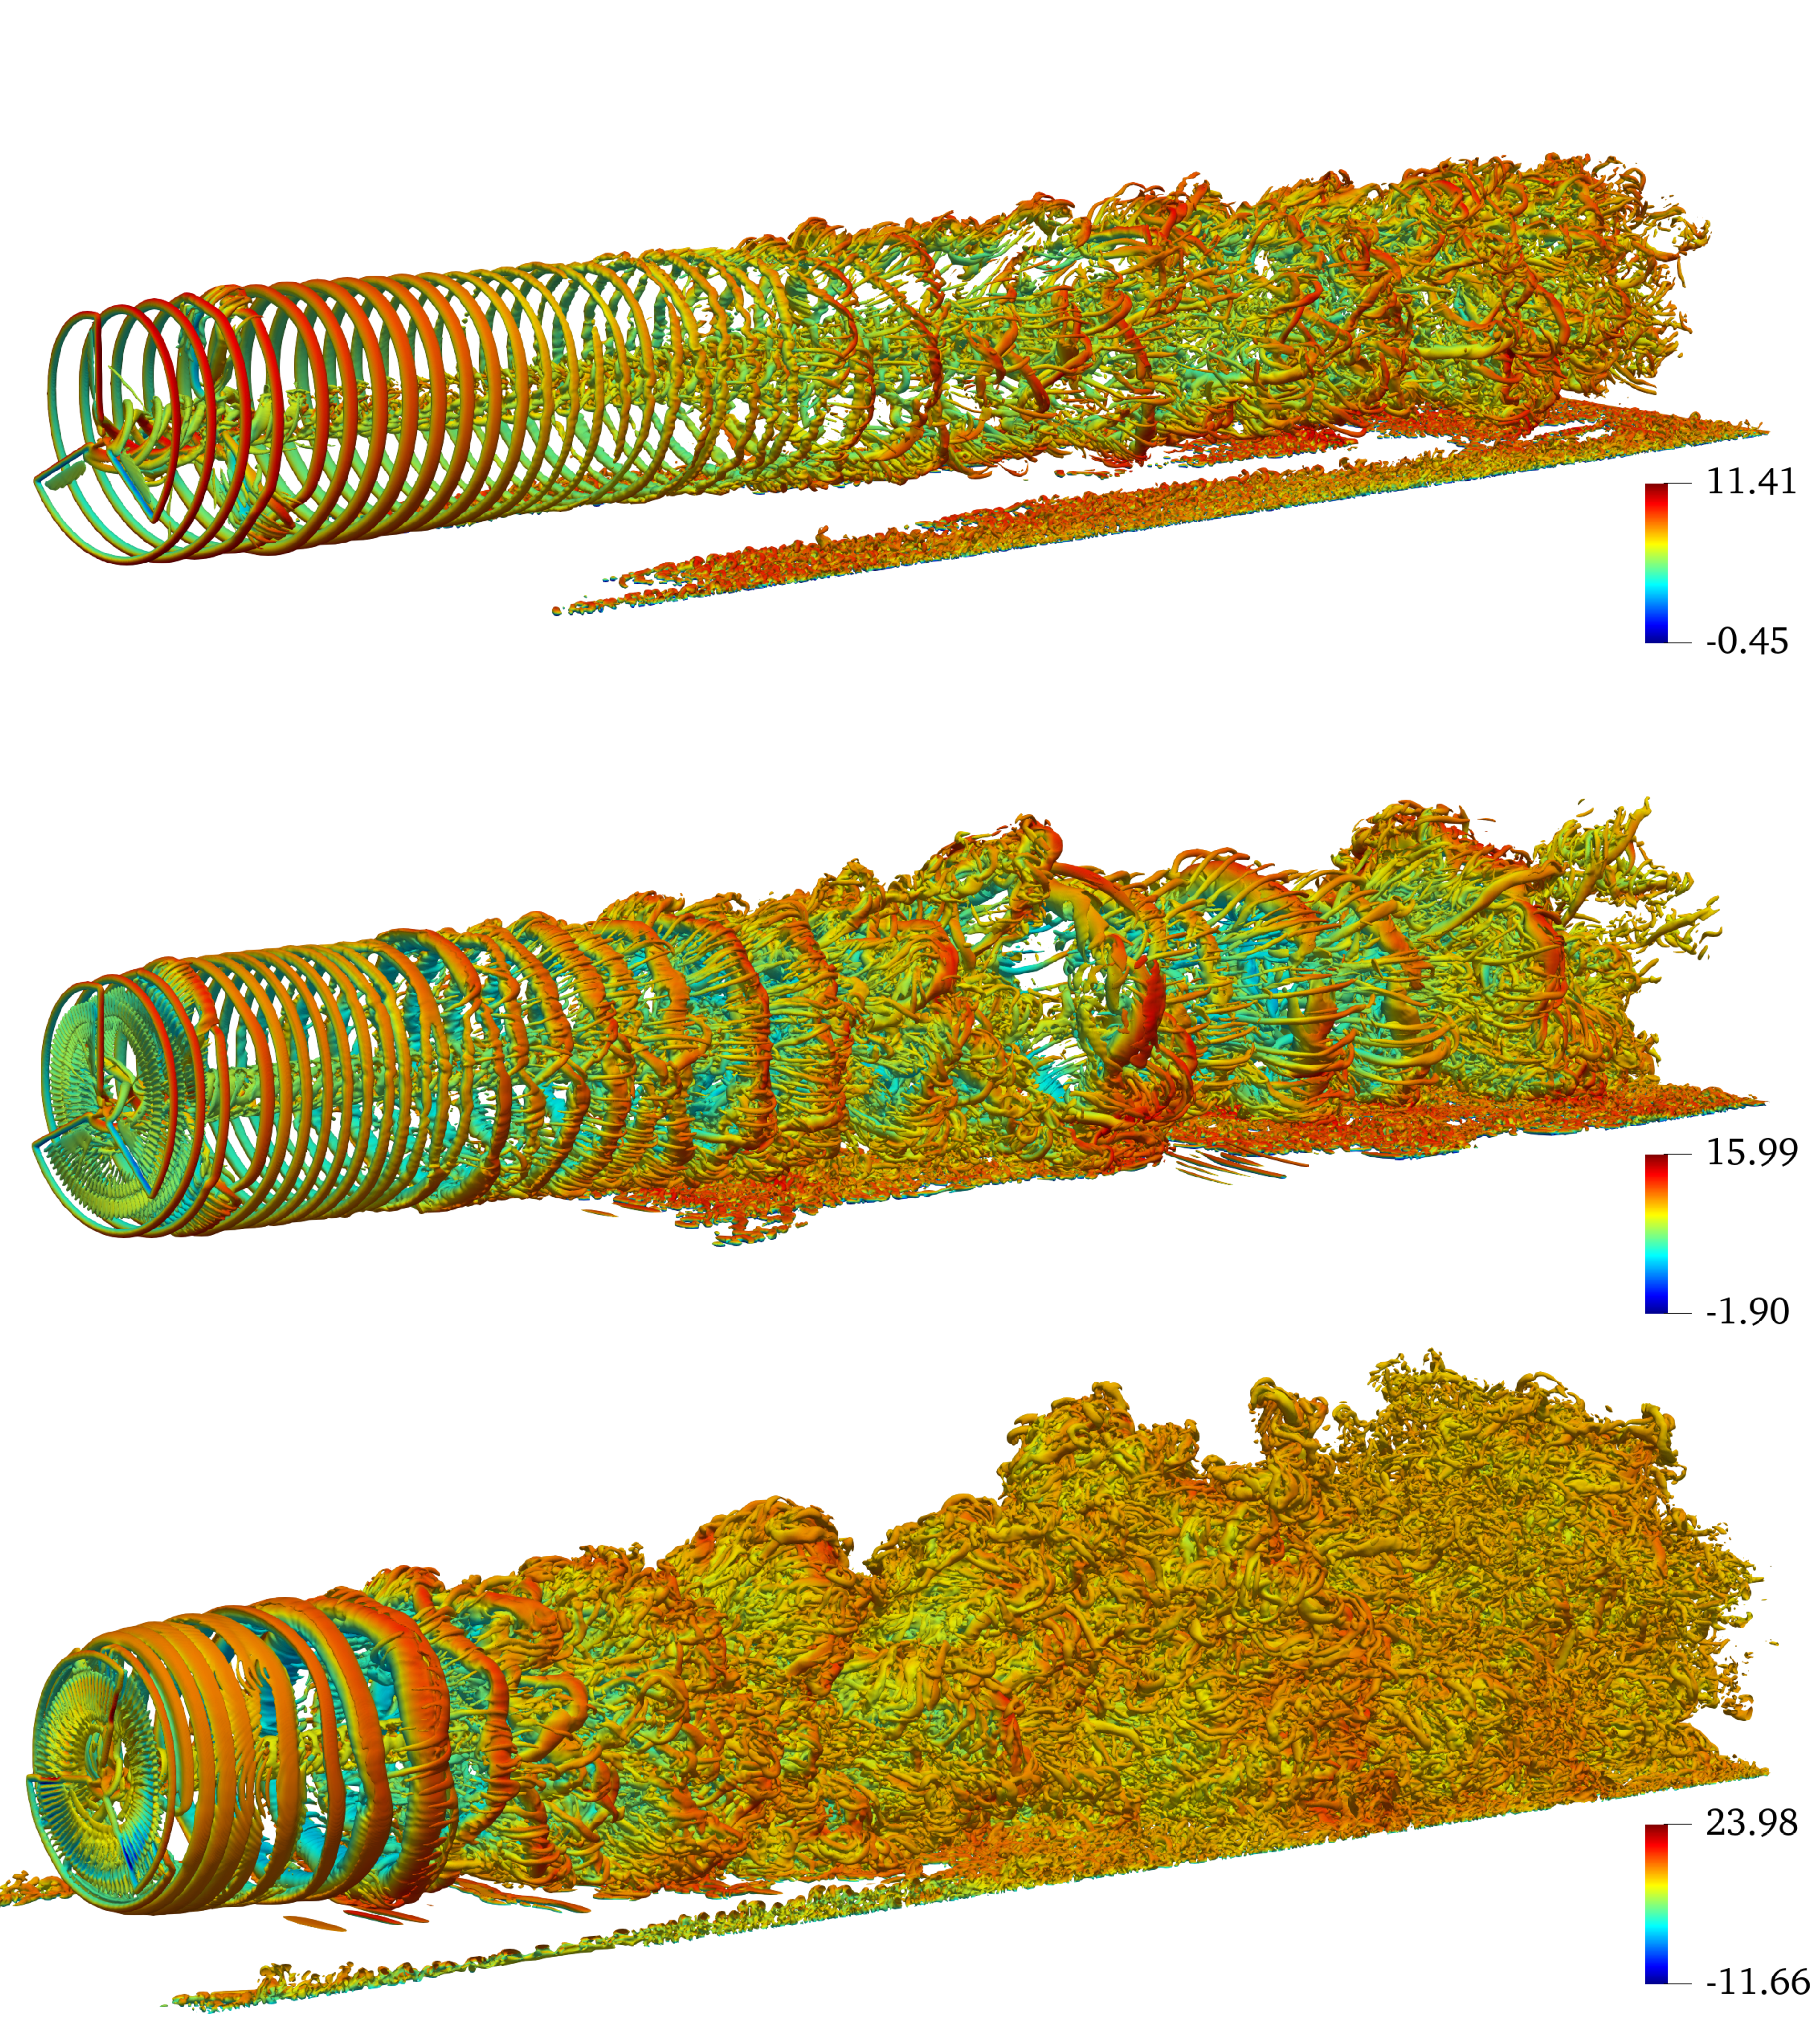
\includegraphics[height=0.8\textheight]{./figs/comp-tsr.pdf}};
\node[text width=5cm,align=left] at (-1,5.8) {{\color{um6pcolor} \Huge TSR = 06}};
\node[text width=5cm,align=left] at (-1.8,5.0) {\small $\mathcal{U}_\infty=08$ [m/s] \& $\omega= 0.762$ [rad/s]};

\node[text width=5cm,align=left] at (-1,3.3) {{\color{um6pcolor} \Huge TSR = 08}};
\node[text width=5cm,align=left] at (-1.8,2.5) {\small $\mathcal{U}_\infty=10$ [m/s] \& $\omega= 1.270$ [rad/s]};

\node[text width=5cm,align=left] at (-1,0.8) {{\color{um6pcolor} \Huge TSR = 13}};
\node[text width=5cm,align=left] at (-1.8,0.0) {\small $\mathcal{U}_\infty=12$ [m/s] \& $\omega= 2.476$ [rad/s]};

\node[text width=11cm,align=left] at (1.5,7.1) {Helicoidal wake structure through instantaneous contours of $Q_{\text{criterion}}$};
\end{tikzpicture}
\end{figure}
\end{frame}


\subsection{Future work}

\begin{frame}{Future work}
\justifying
This simulation framework can be used for more complex configurations. It would be great if we could make progress on the following tasks:

\begin{itemize}
\justifying
\item[\large\ding{236}] Improve coupling implementation (optimization of MPI communications and memory usage) of ALM data structure.
\item[\large\ding{236}] Multiple rotors: analysis of the interaction of the wake on blade deformation turbulence injection.
\item[\large\ding{236}] Simulate the flow around an entire wind farm and assess the inflow's impact.
\end{itemize} 
\end{frame}

\begin{frame}{}
\begin{center}
\Huge\bf Thanks for listening!\\
\end{center}


\end{frame}


\end{document}
